\documentclass[a4paper,10pt]{article}
%%%%%%%%%%% Package %%%%%%%%%%%
\usepackage{amssymb}  % Used for math symbols.
\usepackage{amsmath}  % Used for math environments.
\usepackage[french,english]{babel} % Used to define the language.
\usepackage{datetime} % Used for the dynamic date.
\usepackage{float}    % Used to force figure to stay on place with [H]
\usepackage[T1]{fontenc} % Used to display french character correctly.
\usepackage{geometry} % Used to change margin.
\usepackage{graphicx} % Used to display image/graphic.
\usepackage{hyperref} % Used for hypertext.
\usepackage{inputenc} % Used to specify encodage.
\usepackage{listings} % Used to display code.
\usepackage{lipsum}   % Used to generate lorem ipsum
\usepackage{setspace} % Used to define space betweenbiais  lines.
\usepackage{tabularx} % Used for some table

%%%%%%%%%%% Param %%%%%%%%%%%
\geometry{top=2.4cm, bottom=2.4cm, left=2.4cm , right=2.4cm}
\hypersetup{
    colorlinks=true,            % Color link instead of framing links.
    linkcolor=blue,             % Color of intern link.
    urlcolor=blue,              % Color of url link.
}
\inputencoding{utf8}            % Define the encoding as utf8.
\lstset{
  language={}, % Aucun langage spécifique
  basicstyle=\tt\footnotesize, % Police de caractères // \tt\footnotesize
  numbers=left, % Numérotation des lignes à gauche
  numberstyle=\tiny, % Style de numérotation des lignes // \tiny\color{mygray}
  frame=single, % Encadrement du code
  breaklines=true, % Saut de ligne automatique
  showstringspaces=false % Ne pas afficher les espaces dans les chaînes de caractères
}
\setlength{\parindent}{15pt}    % Define indentation size (default=15pt)
\setstretch{1}                  % Define space between lines (default=1)

%%%%%%%%%%% Useful link %%%%%%%%%%%
% https://www.tablesgenerator.com/ % Useful to create LaTeX table
 
%%%%%%%%%%% Commands %%%%%%%%%%%
\newcommand{\HRule}{\rule{\linewidth}{0.5mm}} % Print a line
\newcommand{\schoolyear}{\the\numexpr\year-(\ifnum\month<9 1\else 0\fi)\relax-\the\numexpr\year+(\ifnum\month<9 0\else 1\fi)} % Print the current academic year.

%%%%%%%%%%% Document %%%%%%%%%%%
\begin{document}

%%%%%%%%%%% Front page %%%%%%%%%%%
\begin{titlepage}
   \begin{center}

    % Upper part of the page. The '~' is needed because 
    % only works if a paragraph has started.
    ~\\[4cm]
    
\includegraphics[scale=0.9]{images/facsa.png}
    ~\\[1.5cm]
    % Title
    \HRule \\[0.4cm]
    {\huge Introduction to Machine Learning\\[0.4cm] }

    \HRule \\[1cm]
    
    \textsc{\Large Bias and variance analysis}\\[2cm]
    \vspace{2cm}
    % Author and supervisor
    \begin{minipage}{0.3\textwidth}
      \begin{flushleft} \large
        Arthur \textsc{GRAILLET}
        Robin \textsc{FONBONNE}
        Thomas \textsc{ROTHEUDT}
      \end{flushleft}
    \end{minipage}
    \begin{minipage}{0.3\textwidth}
      \begin{flushright}\large
        s182019
        s182200
        s191895
      \end{flushright}
    \end{minipage}

    \vfill

    % Bottom of the page
    {\large Academic year \schoolyear}

  \end{center}
\end{titlepage}
\newpage

%%%%%%%%%%% Report %%%%%%%%%%%

%%% Question 1: Analytical derivations
\section{Analytical derivations}
\begin{enumerate}
    %% Question 1.1: Show that the expected generalization error...
    \item 
    We have the expected generalization error of the k-Nearest Neighbours algorithm:
    $$
    E_{LS}\{E_{y\mid \textbf{x}}\{(y - \hat{y}(\textbf{x};LS,k))^2\}\}
    $$
    
    We can substitude $y$ by $f(\textbf{x}) + \epsilon$ and expand the square in the expected squared error written as
    $$
    E_{y\mid \textbf{x}}\{(y - \hat{y}(\textbf{x};LS,k))^2\}
    $$
    to obtain:
    $$
    E_{y\mid \textbf{x}}\{(f(\textbf{x}) - \hat{y}(\textbf{x};LS,k))^2 + 2\epsilon(f(\textbf{x})-\hat{y}(\textbf{x};LS,k)) + \epsilon^2\}
    $$

    Since $E[\epsilon] = 0$ and $\epsilon$ is independent of $f(x)$ and $\hat{y}(\textbf{x};LS,k)$ the cross-term vanishes and the formula becomes:
    $$
    E_{y\mid \textbf{x}}\{(y - \hat{y}(\textbf{x};LS,k))^2\} = (f(\textbf{x})-\hat{y}(\textbf{x};LS,k))^2 + E[\epsilon^2]
    $$

    Since $\epsilon \sim \mathcal{N}(0, \sigma^2)$, we have $E[\epsilon^2] = \sigma^2$ it can be written as:
    $$
    (f(\textbf{x})-\hat{y}(\textbf{x};LS,k))^2 + \sigma^2
    $$

    We can rewrite $\hat{y}(\textbf{x};LS,k)$ as the average of the function values at the k-nearest neighbors:
    $$
    \hat{y}(\textbf{x};LS, k) = \frac{1}{k}\sum^k_{l=1}y_{(l)}
    $$
    where $y_{(l)} = f(\textbf{x}_{(l)}) + \epsilon$ (with $\epsilon \sim \mathcal{N}(0, \sigma^2)$). Therefore it can be written as:
    $$
    \hat{y}(\textbf{x};LS, k) = \frac{1}{k}\sum^k_{l=1}f(\textbf{x}_{(l)}) + \epsilon = \frac{1}{k}\sum^k_{l=1}f(\textbf{x}_{(l)}) + \frac{1}{k}\sum^k_{l=1}\epsilon
    $$

    The expected squared error can be decomposed as follows:
    $$
    \sigma^2  
    + \left(f(\textbf{x})-\frac{1}{k}\sum^k_{l=1}f(\textbf{x}_{(l)})\right)^2
    + 2\left(f(\textbf{x})-\frac{1}{k}\sum^k_{l=1}f(\textbf{x}_{(l)})\right) \left(\frac{1}{k}\sum^k_{l=1}\epsilon\right)
    + \left(\frac{1}{k}\sum^k_{l=1}\epsilon\right)^2
    $$
    Since $\epsilon$ is an independent random variable with a mean of zero, the cross-term has an expectation of zero. We can write the expected generalization error as:
    $$
    E_{LS}\{E_{y\mid \textbf{x}}\{(y - \hat{y}(\textbf{x};LS,k))^2\}\} =
    E_{LS}\left(\sigma^2\right)
    + E_{LS}\left[\left(f(\textbf{x})-\frac{1}{k}\sum^k_{l=1}f(\textbf{x}_{(l)})\right)^2\right]
    + E_{LS}\left[\left(\frac{1}{k}\sum^k_{l=1}\epsilon\right)^2\right]
    $$

    The expectation of a constant is the constant itself and the expectation of the third term
    $$
    E_{LS}\left[\left(\frac{1}{k}\sum^k_{l=1}\epsilon\right)^2\right] = \frac{\sigma^2}{k}
    $$
    because $\text{Var}(\epsilon) = \sigma^2$.

    Since \textbf{x} is fixed, the second term is also fixed. Taking the expectation $E_{LS}$ over this term has no effect.

    Therefore we can conclude that
    $$
    E_{LS}\{E_{y\mid \textbf{x}}\{(y - \hat{y}(\textbf{x};LS,k))^2\}\} =
    \sigma^2
    + \left[f(\textbf{x})-\frac{1}{k}\sum^k_{l=1}f(\textbf{x}_{(l)})\right]^2
    + \frac{\sigma^2}{k}
    $$

    The first term represents the noise, the second the bias, and the third the variance. 

    %% Question 1.2: Let us now assume that the problem is unidimensional...
    \item 
    We know that $f(x) = x^2$. Since we have to evaluate the bias and variance at $x = 0$ we know that $f(x) = 0$.

    The bias can be written as:
    $$
    \text{bias} = \left(\frac{1}{k}\sum^k_{l=1}({x}_{(l)})^2\right)^2
    $$
    Since the training inputs are symmetrically distributed around $x=0$ on a uniform grid in [-1,+1], the k-neighbors of $x=0$ include the point $x=0$, $k'$ positive points, and $k'$ negative points. We have that
    $$
    \sum^k_{l=1}({x}_{(l)})^2 = 2\sum^{k'}_{l=1}\left(\frac{i}{N'}\right)^2 = \frac{2}{(N')^2}\sum^{k'}_{l=1}i^2
    $$
    We can use the formula to write the sum as a function of $k'$:
    $$
    \frac{2}{(N')^2}\sum^{k'}_{l=1}i^2 = \frac{2}{(N')^2}\frac{k'(k'+1)(2k'+1)}{6}
    $$
    The result must be expressed as a function of k and N, we can replace $k'$ and $N'$ with the relation $k' = \frac{k-1}{2}$ and $N' = \frac{N-1}{2}$:
    $$
    \frac{2}{\frac{(N-1)^2}{4}}\frac{(\frac{k-1}{2})(\frac{k-1}{2}+1)(k-1+1)}{6} = \frac{4k(k-1)(\frac{k-1}{2}+1)}{3(N-1)^2}
    $$
    The bias can be written as a function of k and N:
    $$
    \text{bias} = \left(\frac{1}{k}\frac{4k(k-1)(\frac{k-1}{2}+1)}{3(N-1)^2}\right)^2 =  \left(\frac{4(k-1)(\frac{k-1}{2}+1)}{3(N-1)^2}\right)^2 
    $$


    The variance is already expressed as a function of $\sigma$ and $k$:
    $$
    \text{variance} = \frac{\sigma^2}{k}
    $$

    
    %% Question 1.3: Discuss the impact of N, k, an σ on bias and variance. Are there 
    % some surprising or missing dependences? If so, try and explain them.
    \item 
    \begin{itemize}
        \item 
        $k$ appears in the formula of the variance and it is obvious that a greater k leads to a smaller variance. But increasing $k$ may lead to an increase of the biais because we would consider more distant points which reduce the flexibility of the model.
        \item
        Increasing the size $N$ of the learning sample generally leads to a denser distribution, therefore with the same $k$ and $\sigma$, the k-nearest neighbors around $x$ will be closer to $x$ and we can expect that they better represent the local behavior of $f(x)$.
        We can say that larger N leads to smaller bias. If we consider the problem explain in 2, we can see that the size $N$ is in the bias formula and increasing $N$ reduces the bias.

        $N$ has no direct impact on the variance but we can note that a larger $N$ allows a larger $k$ which leads to a lower variance. 
        \item 
        A greater $\sigma$ means more noise and as we may expect it increases the variance but does not impact the biais.
    \end{itemize}


    
    %% Question 1.4: For all combinations of N in {25, 50} and σ ∈ {0.0, 0.1, 0.2}, determine 
    % the value k∗ of k that minimizes the expected generalization error at x = 0.
    \item
    As suggested we'll compute the minimum by running actual experiments. We have to minimize this function:
    $$
    f(k) = \sigma^2 + \left[\frac{-(k^2 - 1)}{3(N-1)^2}\right]^2 + \frac{\sigma^2}{k}
    $$
    By testing every possible value of $k$ such that $k = 2k' + 1$ with $0 \le k' \le \frac{N-1}{2}$ for each combination of $N$ and $\sigma$ we have the following results:
    \begin{table}[H]
      \centering
      \begin{tabular}{l|l|l|l|}
      \cline{2-4}
                               & $\sigma = 0$ & $\sigma = 0.1$ & $\sigma = 0.2$ \\ \hline
      \multicolumn{1}{|l|}{$N = 25$} & 1  &  5  &  7 \\ \hline
      \multicolumn{1}{|l|}{$N = 50$} & 1  &  11   &  13 \\ \hline
      \end{tabular}
      \caption{Table of $k^*$ considering only odd values for k}
    \end{table}
    The cells represent the $k^*$ for each combination.

    If we can still consider even values for $k$ with the formula obtained considering only odd values of $k$ we would have:
    \begin{table}[H]
      \centering
      \begin{tabular}{l|l|l|l|}
      \cline{2-4}
                               & $\sigma = 0$ & $\sigma = 0.1$ & $\sigma = 0.2$ \\ \hline
      \multicolumn{1}{|l|}{$N = 25$} & 1  &  6  &  8 \\ \hline
      \multicolumn{1}{|l|}{$N = 50$} & 1  &  11   &  14 \\ \hline
      \end{tabular}
      \caption{Table of $k^*$ considering every value for $k$}
    \end{table}

    % It was an atttempt at the derivative approach:
    % As suggested we'll compute the minimum of the bias plus variance found in 2. Let's define:
    % $$
    % f(k) = \sigma^2 + \left[\frac{-(k^2 - 1)}{3(N-1)^2}\right]^2 + \frac{\sigma^2}{k}
    % $$
    % To find the minimum we should first compute the derivative $f'(k)$:
    % $$
    % f'(k) = \frac{4k(k^2-1)}{9(N-1)^4} - \frac{\sigma^2}{k^2}
    % $$
    % The term with the greastest ordre of $k$ (third order) in $f(k)$ is positive and $f(k)$ is continuous, 
    % therefore the minimum occurs when the derivative is null.
    % $$
    % f'(k) = 0
    % $$
    % We find:
    % $$
    % k = pas trouvé
    % $$
    % This doesn't take into account that k must be an integer nor the fact that the formula were found assuming k being odd.

    % The results using the derivative are the following:
    % \begin{table}[H]
    %   \centering
    %   \begin{tabular}{l|l|l|l|}
    %   \cline{2-4}
    %                            & $\sigma = 0$ & $\sigma = 0.1$ & $\sigma = 0.2$ \\ \hline
    %   \multicolumn{1}{|l|}{$N = 25$} & 0  &  1,423  &  2,258 \\ \hline
    %   \multicolumn{1}{|l|}{$N = 50$} & 0  &  2,290   &  3,635 \\ \hline
    %   \end{tabular}
    %   \caption{Table of $k^*$ based on derivative}
    % \end{table}
    % These values cannot be used like that for as an hyperparameter. We have to consider at least one neighbor and the float must be rounded to integer.

    % If we compute the best $k*$ using experiments with only odd values of $k$ we find the following results:
    % \begin{table}[H]
    %   \centering
    %   \begin{tabular}{l|l|l|l|}
    %   \cline{2-4}
    %                            & $\sigma = 0$ & $\sigma = 0.1$ & $\sigma = 0.2$ \\ \hline
    %   \multicolumn{1}{|l|}{$N = 25$} & 1  &  3  &  3 \\ \hline
    %   \multicolumn{1}{|l|}{$N = 50$} & 1  &  3   &  5 \\ \hline
    %   \end{tabular}
    %   \caption{Table of $k^*$ based on experiments}
    % \end{table}


    %% Question 1.5: Discuss the impact of N and σ on k∗.
    \item 
    Increasing the size of $N$ or $\sigma$ tends to increase the value of $k^*$. If $\sigma = 0$ then modifying $N$ won't change $k^*$ because the best value would always be to consider only one element.
\end{enumerate}

%%% Question 2: Empirical analysis
\section{Empirical analysis}
    %% Question 2.1: Explain why estimating the residual error term is very difficult in this setting.

\subsection{}

The residual error represents the minimal attainable error, which is the irreducible noise in the data. The key challenge is that we don't know the true function $f^*(x)$ that maps wine characteristics to quality scores. Without this true function $f^*(x)$, we cannot measure how much of the prediction error comes from noise versus other sources of error.
    
    This is because the residual error is defined as the difference between the actual observed values y and the true function values \[ f^*(x): \mathbb{E}[(y - f^*(x))^2]\]
    Even if we build a very good model, we cannot know how close it is to this true underlying function f*(x), and therefore cannot isolate how much of the error is truly irreducible (residual error) versus due to model imperfections. 
    
    In our case, this is particularly challenging because the relationship between wine characteristics and quality involves human judgments that do not follow any consistent mathematical function, making the true $f^*(x)$ even more difficult to determine. 
    
    Additionally, the observed error is a combination of bias, variance, and residual error. \[ Total Error = Bias + Variance + ResidualError\] Since bias and variance arise from model imperfections, separating these components from the irreducible residual error becomes nearly impossible without further assumptions or prior knowledge of the noise distribution.
    

    %% Question 2.2: Describe a protocol to nevertheless estimate variance, the expected error, as 
    % well as the sum of the bias and the residual error from a pool P.

\subsection{}

The objective of our protocol is to decompose the total error of a model into three components:
\begin{itemize}
    \item \textbf{Total Error (Expected Error)}: The mean squared difference between predictions and true values.
    \item \textbf{Variance}: Variability in predictions due to the randomness of training samples.
    \item \textbf{Bias Squared + Residual Error}: Systematic error due to the difference between the model's average prediction and the true values, plus the irreducible error.
\end{itemize}

\begin{enumerate}
    \item \textbf{Dataset Preparation}: Split the dataset into two subsets: 
    \begin{itemize}
        \item \textbf{Training set (80\%)}: Used for creating subsamples.
        \item \textbf{Test set (20\%)}: Fixed and used to evaluate all models.
    \end{itemize}

    \item \textbf{Subsample Generation}: 
    \begin{itemize}
        \item Define the subsample size ($\mathbf{N}$) for each training subset (e.g., $\mathbf{N}$=250).
        \item Create multiple subsamples (e.g., 80) from the training set by randomly sampling without replacement. These subsamples simulate diverse training conditions, reflecting real-world variability.
    \end{itemize}

    \item \textbf{Train Models on Subsamples}
    \begin{enumerate}
        \item For each training subset:
        \begin{enumerate}
            \item Train a model using the subset.
            \item Make predictions on the fixed test set.
        \end{enumerate}
        \item Store the predictions in a matrix of size \(M \times N_{\text{test}}\), where:
        \begin{itemize}
            \item \(M\): Number of subsamples.
            \item \(N_{\text{test}}\): Number of test instances.
        \end{itemize}
    \end{enumerate}

   \item \textbf{Compute Metrics}
\begin{enumerate}
    \item \textbf{Total Error:} The expected squared difference between the mean prediction and the true values:
    \[
    \text{Total Error} = \mathbb{E}\left[(\mathbb{E}[\hat{y}] - y)^2\right]
    \]
    where:
    \begin{itemize}
        \item \(\hat{y}\): Prediction for a given test instance.
        \item \(y\): True value for the same test instance.
    \end{itemize}

    \item \textbf{Variance:} The expected variability of predictions across subsamples:
    \[
    \text{Variance} = \mathbb{E}\left[\text{Var}(\hat{y})\right]
    \]
    where:
    \begin{itemize}
    \item \(\text{Var}(\hat{y}) = \frac{1}{M} \sum_{j=1}^{M} \left(\hat{y}_j - \frac{1}{M} \sum_{k=1}^{M} \hat{y}_k \right)^2\): 
    Variance of predictions across different subsamples for a given test instance.
    \item \(M\): Number of subsamples used in the calculation.
    \item \(\hat{y}_j\): Prediction from the \(j\)-th model (trained on the \(j\)-th subsample).
    \item \(\frac{1}{M} \sum_{k=1}^{M} \hat{y}_k\): Mean prediction across all subsamples for a given test instance.
\end{itemize}


    \item \textbf{Bias + Residual Error:} The remaining error after accounting for variance:
    \[
    \text{Bias}^2 + \text{Residual Error} = \text{Total Error} - \text{Variance}
    \]
    where:
    \begin{itemize}
        \item \(\text{Bias}^2\): Systematic difference between the expected prediction and the true value.
        \item Residual Error: The irreducible error inherent to the problem.
    \end{itemize}
\end{enumerate}


    \item \textbf{Hyperparameter Exploration}
    \begin{itemize}
        \item Repeat Steps 2--4 for different values of the model's complexity parameter:
        \begin{itemize}
            \item \textbf{kNN:} Number of neighbors (\(k\)).
            \item \textbf{Lasso:} Regularization strength (\(\lambda\)).
            \item \textbf{Decision Tree:} Maximum depth.
        \end{itemize}
    \end{itemize}
    
\end{enumerate}
    
 %% Question 2.3: Implement and use this protocol on the given dataset to estimate the expected error, 
% variance, and the sum of bias and residual error, for Lasso regression, kNN, and regression trees.
\subsection{}

For this experiment, we fixed the learning sample size to 250 and varied the number of learning samples. We evaluated the expected error, variance, and the sum of bias and residual error for three different models: k-Nearest Neighbors, Lasso regression, and Regression Trees. We plotted the evolution of these quantities as a function of the main complexity parameter for each model.

\subsubsection{kNN}

\begin{figure}[H]
    \centering
    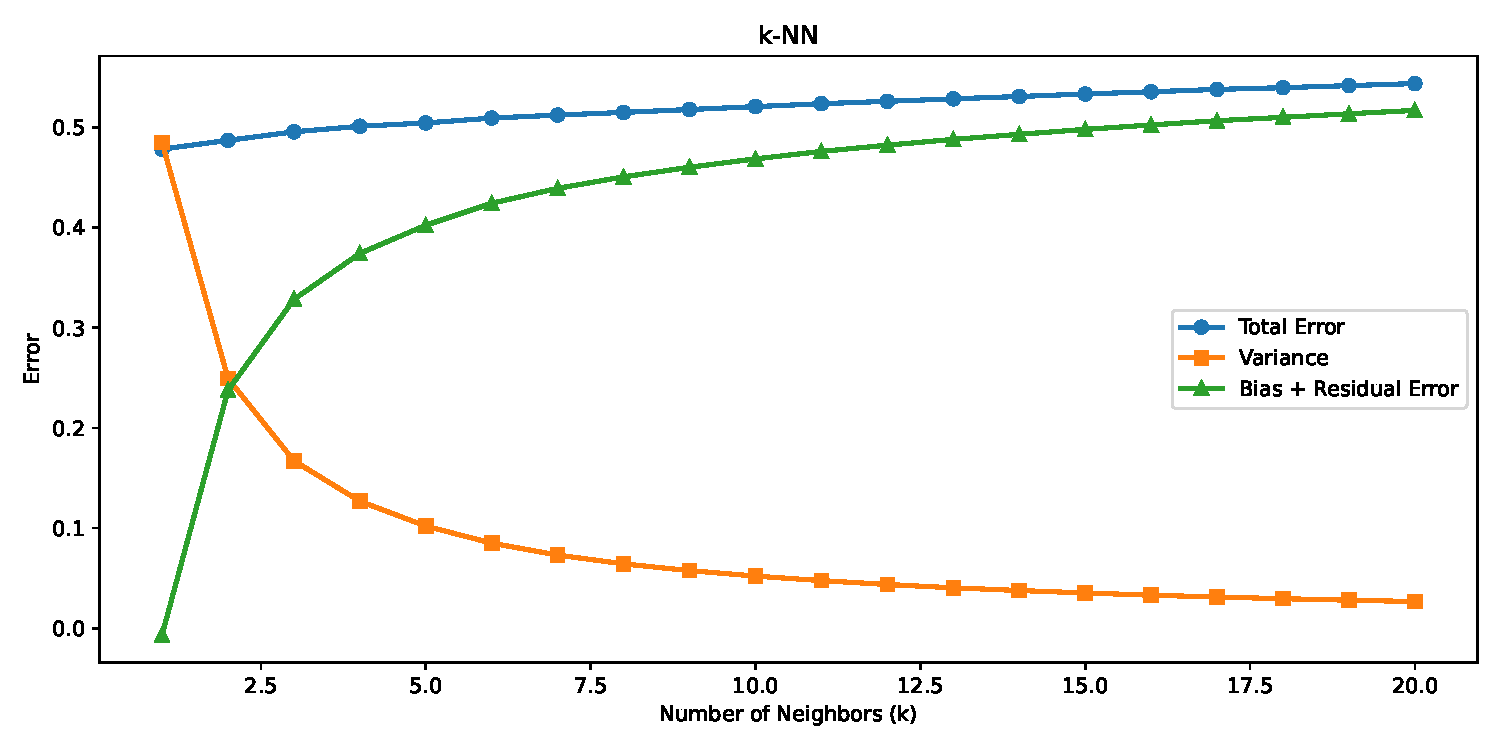
\includegraphics[width=0.8\linewidth]{images/2.3_knn.pdf}
\end{figure}

Discussion:

For k-NN, we varied the number of neighbors (\(k\)) from 1 to 20. The \textbf{Total Error} decreases sharply as \(k\) increases from small values, indicating improved model performance as more neighbors are incorporated into the predictions. This reflects that averaging over more neighbors reduces the model’s sensitivity to noise and outliers. However, beyond a certain point, the total error stabilizes, as the reduction in variance is offset by an increase in bias. This behavior is consistent with the bias-variance trade-off.

The \textbf{Variance} decreases as \(k\) increases because the model becomes less sensitive to individual data points. For small values of \(k\), the predictions rely heavily on the nearest training points, resulting in high variance. As \(k\) grows, the predictions are averaged over more neighbors, reducing the variability in the predictions and smoothing the model's output. This reduction in variance demonstrates the model's increasing robustness to noise.

The \textbf{Bias + Residual Error} increases with \(k\). When \(k\) is small, the model is highly flexible, capturing fine-grained details in the data, leading to low bias. As \(k\) increases, the model oversmooths the data, failing to capture finer patterns, and the bias grows. The residual error remains constant as it is intrinsic to the data and independent of the model's complexity.


\subsubsection{Lasso}

\begin{figure}[H]
    \centering
    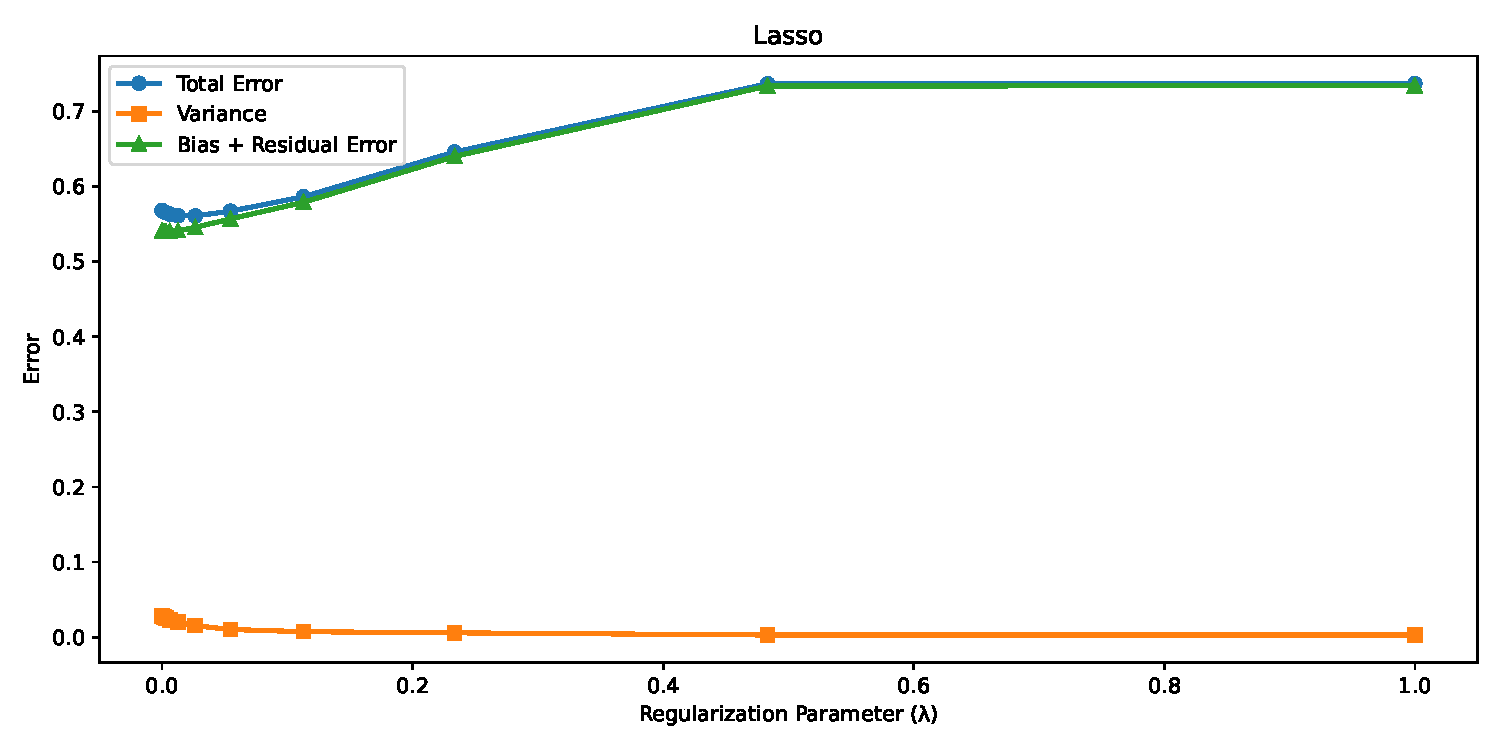
\includegraphics[width=0.8\linewidth]{images/2.3_lasso.pdf}
\end{figure}

Discussion:

For Lasso regression, we varied the regularization parameter \(\lambda\) on a logarithmic scale, ranging from \(10^{-6}\) to \(10^0\). The graph shows the behavior of the total error, variance, and the sum of bias and residual error as \(\lambda\) increases.

As \(\lambda\) increases, the \textbf{Total Error} (blue curve) gradually rises. This behavior indicates that the model becomes too simplistic, leading to underfitting. The increase in \(\lambda\) penalizes the magnitude of the model’s coefficients, forcing them towards zero. While this reduces overfitting, it also limits the model’s flexibility to fit the data, causing it to miss important patterns and increasing the error.

The \textbf{Variance} (orange curve) decreases sharply as \(\lambda\) increases. This is because the regularization term suppresses large coefficients, making the model less sensitive to small fluctuations or noise in the training data. A smaller variance implies that the predictions are more stable across different subsets of the data, reflecting the model's reduced sensitivity to overfitting.

On the other hand, the \textbf{Bias + Residual Error} (green curve) increases with \(\lambda\). As the model is regularized more heavily, it becomes overly simplistic and fails to capture the complexity of the underlying data distribution. This behavior exemplifies the classic \textbf{bias-variance trade-off}: higher regularization reduces variance but increases bias.

\subsubsection{Regression Tree}

\begin{figure}[H]
    \centering
    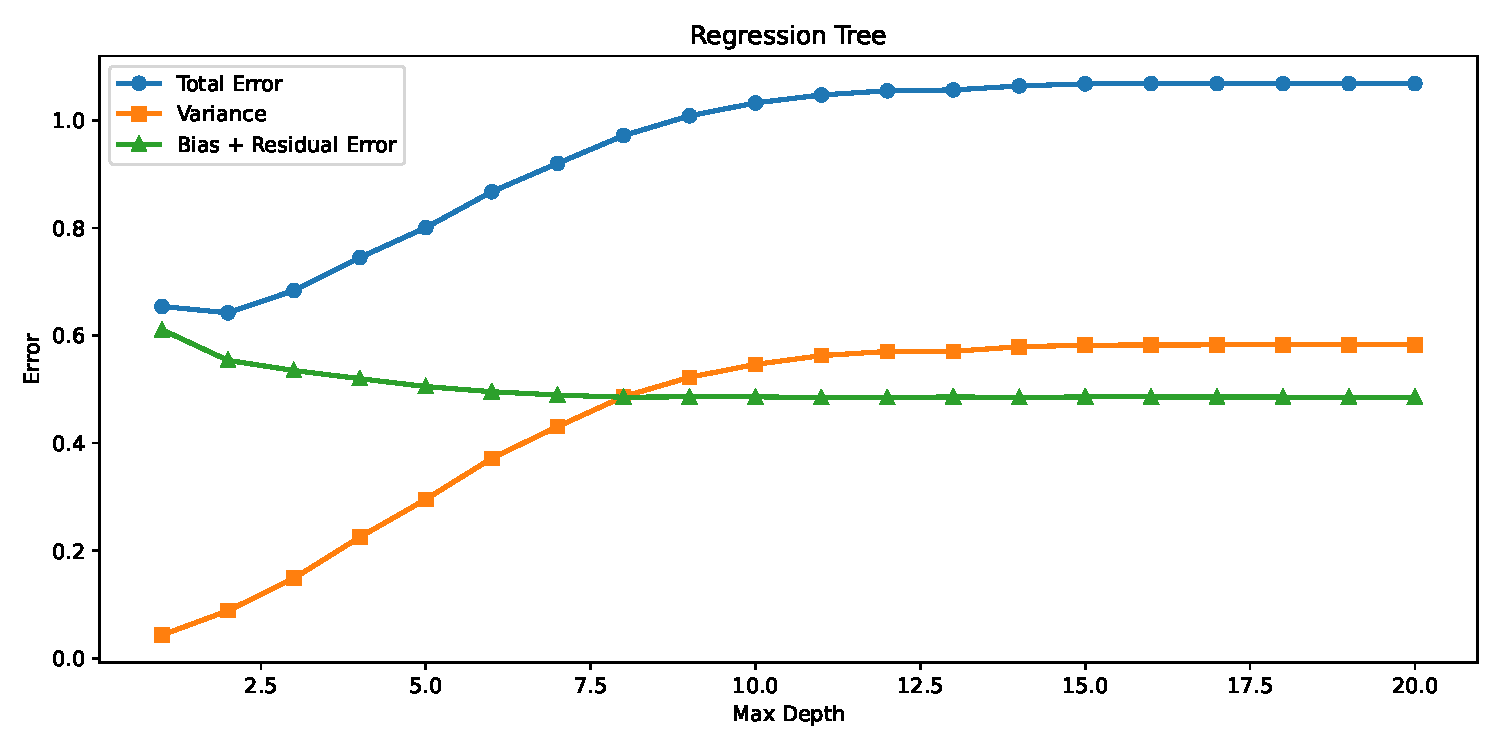
\includegraphics[width=0.8\linewidth]{images/2.3_rt.pdf}
\end{figure}

Discussion:

For Regression Trees, we varied the maximum depth from 1 to 20. Initially, as the depth increases, the \textbf{Total Error} (blue curve) decreases. This indicates that the tree is capturing more complex patterns in the data, improving model performance. However, after reaching an optimal depth, further increasing the depth leads to an increase in total error, as the model starts overfitting the training data. Overfitting occurs because the tree becomes excessively complex and adapts to noise in the data.

The \textbf{Variance} (orange curve) increases with the maximum depth. Deeper trees are more sensitive to the training data, capturing noise and fluctuations, which results in higher variance. This sensitivity causes the model to perform inconsistently across different datasets, reducing its generalization ability.

The \textbf{Bias + Residual Error} (green curve) decreases as the depth increases. Shallow trees have high bias because they are too simple to capture the underlying relationships in the data, leading to systematic errors. As the tree becomes more flexible with increased depth, it models more complex relationships and reduces bias. However, this comes at the cost of increased variance.

This behavior follows the classic \textbf{bias-variance trade-off}: shallow trees exhibit high bias but low variance (underfitting), while deeper trees show low bias but high variance (overfitting). The optimal depth achieves a balance, capturing enough complexity to reduce bias while controlling the variance. Additionally, deeper trees tend to perform better with larger datasets, as they have more information to learn from. However, if the training sample is small, deeper trees are more likely to overfit the data.




    
%% Question 2.4: For the same three methods, show the impact of the learning sample size on bias and 
% variance.

\subsection{}

\subsubsection{kNN - k=5}

\begin{figure}[H]
    \centering
    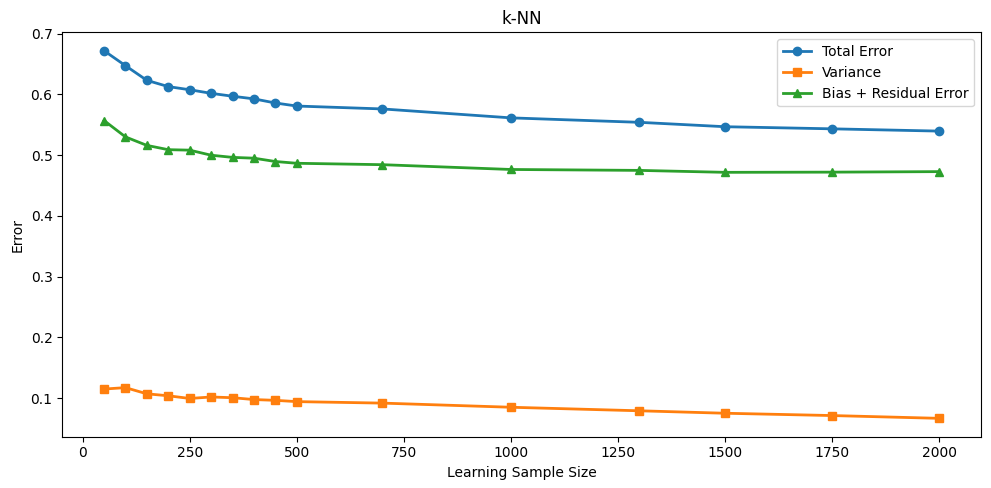
\includegraphics[width=0.8\linewidth]{2.4_knn.png}
\end{figure}

Discussion:  
For kNN, we fixed the number of neighbors to 5 and varied the learning sample size. The plot shows that as the learning sample size increases, the total error decreases, indicating improved model performance with more data. The variance also decreases with increasing sample size, as the model becomes more stable and less sensitive to individual data points. The bias error remains relatively constant, suggesting that the ability of the model to capture the underlying patterns does not change significantly with more data. This behavior aligns with the theory that increasing the sample size reduces variance by providing more information for the model to generalize better, while bias remains relatively unaffected as it is more dependent on the complexity of the model. This highlights the bias-variance trade-off in kNN, where smaller sample sizes lead to higher variance and overfitting, while larger sample sizes help stabilize the model.

\subsubsection{Lasso - $\lambda$ = 0.01 }

\begin{figure}[H]
    \centering
    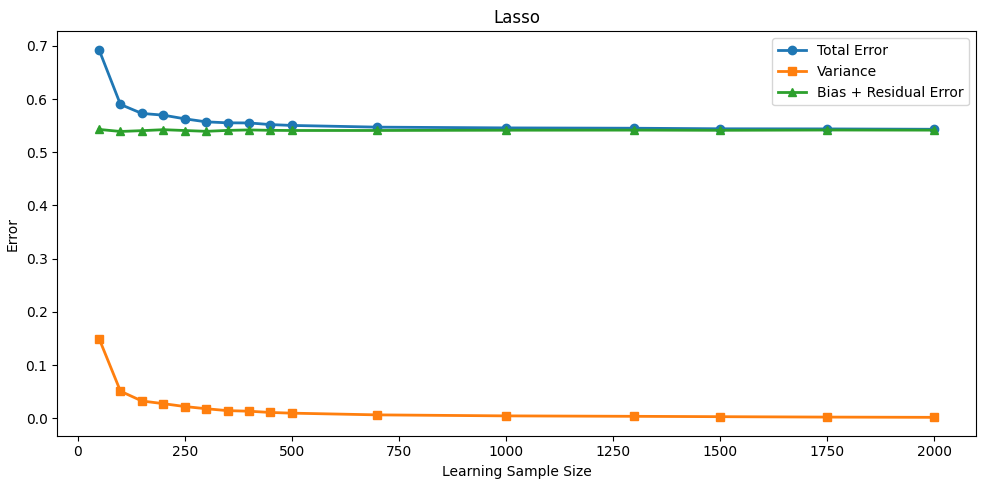
\includegraphics[width=0.8\linewidth]{2.4_lasso.png}
\end{figure}

Discussion:  
For Lasso, we fixed the regularization parameter to 0.01 and varied the learning sample size. The plot shows that as the learning sample size increases, the total error decreases, indicating improved model performance with more data. The variance decreases with increasing sample size as well, as the model becomes more stable and less sensitive to noise in the training set. The bias error remains relatively constant, suggesting that the ability of Lasso to capture the underlying patterns does not change significantly with more data, which is consistent with the fixed regularization parameter. As the sample size increases, the variance decreases due to a more robust coefficient estimation, while the bias remains largely unaffected by sample size, as the regularization strength governs the complexity of the model. This illustrates that the performance of Lasso is more dependent on regularization than on sample size.

\subsubsection{Regression Trees - Fixed Depth}

\begin{figure}[H]
    \centering
    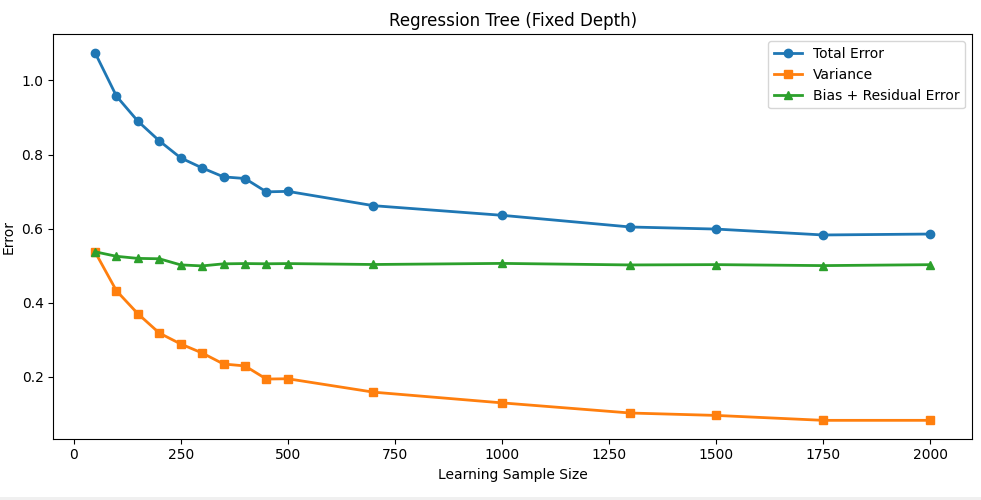
\includegraphics[width=0.8\linewidth]{2.4_rt_fixed.png}
\end{figure}

Discussion:  
For the regression tree with fixed depth, we set the maximum depth to 5 and varied the learning sample size. The plot shows that as the learning sample size increases, the total error decreases, indicating improved model performance with more data. The variance also decreases with increasing sample size as the model becomes more stable and less sensitive to individual data points. The bias error remains relatively constant, suggesting that the tree's ability to capture underlying patterns does not change significantly with more data, as the tree is constrained by its fixed depth. With more data, the model's stability improves, leading to a decrease in variance. However, due to the fixed depth, the bias remains constant, as the model's complexity is predetermined and does not adapt to the data.

\subsubsection{Regression Tree - Full}

\begin{figure}[H]
    \centering
    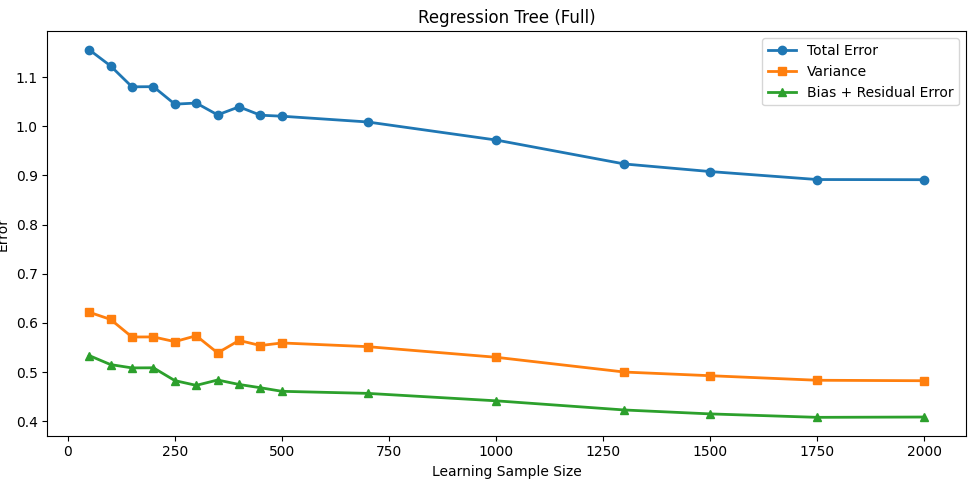
\includegraphics[width=0.8\linewidth]{2.4_rt_full.png}
\end{figure}

Discussion:  
For the regression tree with full depth, we allowed the tree to grow without any depth restriction and varied the learning sample size. The plot shows that as the learning sample size increases, the total error decreases, indicating improved model performance with more data. The variance decreases with increasing sample size, as the model becomes more stable and less sensitive to individual data points. The bias error remains relatively constant, suggesting that the ability of the model to capture the underlying patterns does not change significantly with more data. This behavior aligns with the theory that increasing the sample size reduces variance by providing more information for the model to generalize better, while bias remains relatively unaffected as it is more dependent on the complexity of the model. Unlike the fixed depth tree, the fully grown tree has a lower bias due to its higher flexibility, but it exhibits higher variance, especially when the sample size is small, as it tends to overfit the data. As the sample size increases, overfitting is mitigated, and the model's variance reduces, allowing it to generalize better.



    %% Question 2.5: Two so-called ensemble methods to address variance and bias are bagging 
    % ("bootstrap aggregating") and boosting. 

    
        
\end{document}